\noindent
\rule{0.75\linewidth}{0.3pt}
\section{Threaded elements and screws}
\begin{multicols}{2}
	
	The main dimensions to consider while dealing with threaded elements are the root diameter $d_r$ (inner dimension on the screw), the major nominal diameter $d$ (measured on the external edge) and the pitch (mean) diameter $d_p$. Each thread presents an axial pitch $p$ (distance between contiguous threads), a lead $L$ (travel of a pitch for a round, integer multiple of $p$) and a helix angle $\lambda$ such that $L = \pi d_p \tan\lambda$.\\
	Usually the \textit{inclination} of the thread ($30^\circ$ in the next figure) is described by the parameter $\alpha$.
	
	\begin{center}
		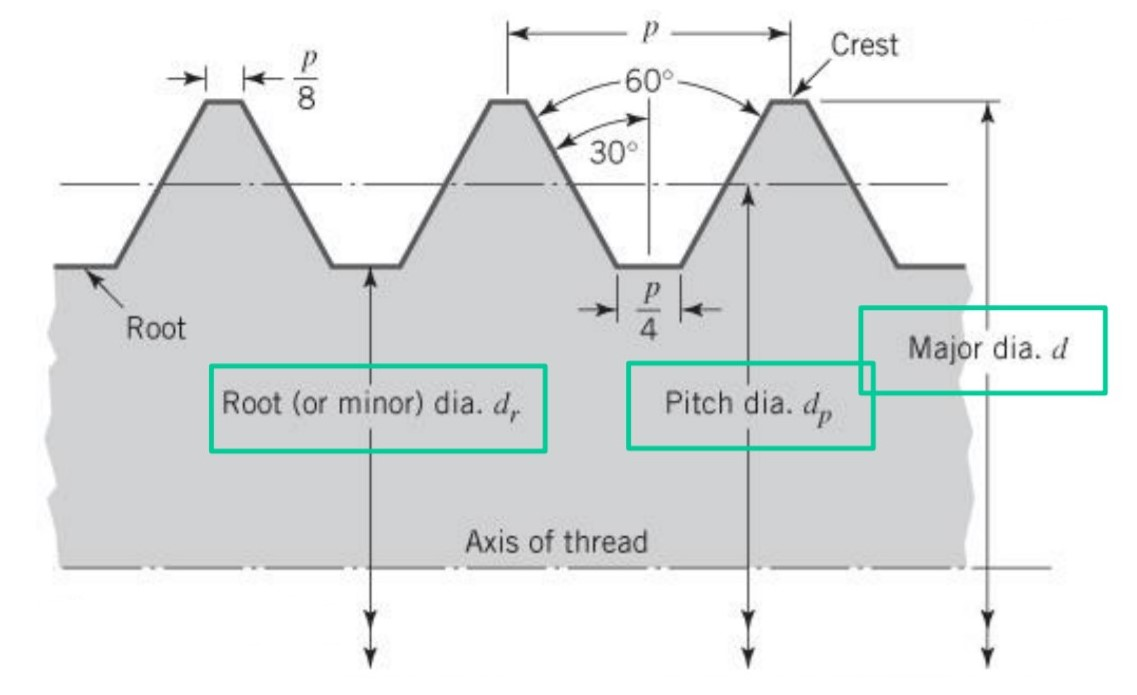
\includegraphics[width=\linewidth]{thread-profile}
	\end{center}
	
	Each standard has it's particular thread profile and values for the various parameters.

	Each screw should be described by a major (nominal) diameter (12), a length (50), a reference standard (ISO 4014) and a property class (8.8) as
	\begin{center}
		Screw \texttt{M12 x 50 ISO 4014-8.8}
	\end{center}
	In particular while defining the property class (according to ISO definitions) the first number is used to express the tensile strength in $100MPa$, while the other number (right side of the point) represent the relative percentage value of the yield strength; in the particular case of class \texttt{ISO 4014-8.8} we have a tensile strength $\sigma_r = 8\cdot 100 MPa$ and a yield of $\sigma_{ys}=0.8 \sigma_r = 640MPa$.
	
	The property class is related to the material of the threaded element, however similar concepts and codes are defined to classify both the head of the screws and the nuts.
	
\subsection{Power screws}
	Power screws use mechanical advantage of the threaded element in order to lift weights.
	\begin{center}
		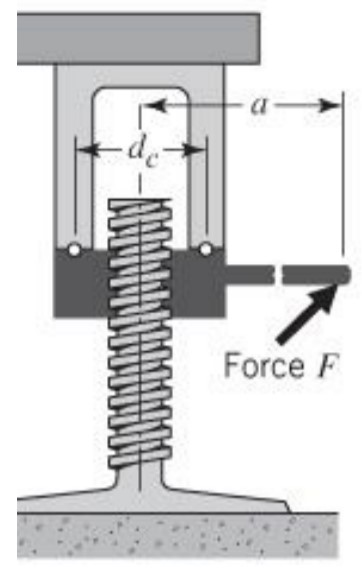
\includegraphics[width=3cm]{power-screw}
	\end{center}
	By doing a force equilibrium it's possible to compute the torque $T$ (determined by the force $F$, so $T=Fa$) that has to be transmitted in order to lift a weight $w$ is determined by the equation
	\begin{equation}
		T = \frac{w d_m}{2} \frac{f\pi d_m + \cos\alpha_n L}{-fL + \pi d_m \cos\alpha_n} + \frac{wf_cd_c}{2}
	\end{equation}
	where $f$ is the friction coefficient between the screw and the collar, $f_c$ the friction coefficient between the collar (having diameter $d_c$) and the support of the weight to be lifted, while the other parameters $\alpha_m,L,d_m$ are specific for the threaded element (as previously defined). Similarly the torque to apply in order to lower the same weight has to be equal to
	\[ T = \frac{w d_m}{2} \frac{f\pi d_m - \cos\alpha_n L}{fL + \pi d_m \cos\alpha_n} + \frac{wf_cd_c}{2} \]
	
	Power screws can be of 2 type: self locking if, with no torque applied, the system stays locked due to the friction contact between the threaded element and the lever, while in the other condition we refer the system as a overhauling screw. The condition on the friction $f$ in order to have a self locking screw is
	\[ f \geq \frac{L\cos\alpha_n}{\pi d_m} = \tan\lambda \, \cos\alpha_n \]
	The efficiency $e$ of the system that determines the ratio of the lifting power respect to the input power (considering that part of the power is dissipated by friction) is equal to
	\[ e= \frac{\cos\alpha_n - f\tan\lambda}{\cos\alpha_n + f\cot \lambda } \]
	
	
	
	
	
	
	
	
	
	
	
	
	
	
	
	
	
	
	
	
	
	
	
	
	
	
	
	
	
	
	
	
	
	
	
	
	
	
	
	
	
	
	
	
	
\end{multicols}